\documentclass[a4paper]{article}

\title{Assignment 4}
\author{Munan Hou}

\usepackage{Sweave}
\begin{document}
\Sconcordance{concordance:Assignment_4.tex:Assignment_4.Rnw:%
1 5 1 1 0 6 1 1 2 1 0 1 1 3 0 1 2 3 1 2 2 5 1}


\maketitle{1. CLT}
I've searched the google and found 10+ tests. The tests that I familiar with are Kolmogorov–Smirnov test, Pearson's chi-squared test, test of kurtosis and skewnessand, and shapiro-wilk test and qq plot.

So I am going to dig this on my own way. This is a little bit mess.

\begin{Schunk}
\begin{Sinput}
> library(ggplot2)
> library(nortest)
> library(normtest)
\end{Sinput}
\end{Schunk}




First, sample and summary that on average, for sums of how many uniform distribution could follow a normal distribution, on the significance level p=.05
\begin{Schunk}
\begin{Sinput}
> data1 <- c()
> number <- c()
> for (k in 1:100) {
+   for (i in 1:50) {
+     data1 <- c()
+     for (j in 1:1000) {
+       index <- runif(i)
+       sumindex <- sum(index)
+       data1[j] <- sumindex
+     }
+     if (shapiro.test(data1)["p.value"] > .05) {
+       number <- c(number,i);break
+     }
+   }
+ }
> number
\end{Sinput}
\begin{Soutput}
  [1] 4 5 3 3 4 3 4 3 4 4 4 4 4 4 4 4 4 5 6 3 4 4 3 4 5 4 3 4 3 4 4 4 4 4 4 4 3
 [38] 3 4 3 3 3 4 3 3 3 3 3 4 6 3 3 4 4 4 3 5 3 4 4 4 4 5 3 3 4 4 4 5 4 3 3 4 5
 [75] 3 3 4 4 4 4 4 3 4 3 4 4 5 6 3 4 5 4 4 3 3 4 4 5 4 3
\end{Soutput}
\begin{Sinput}
> mean(number)
\end{Sinput}
\begin{Soutput}
[1] 3.82
\end{Soutput}
\end{Schunk}
Result shows, on average, the mean of "the sum of minimum amount of uniform distributions" which can construct a normal distribution is approximately 4.

Then test Poisson distribution with lambda = 10.
\begin{Schunk}
\begin{Sinput}
> data1 <- c()
> number <- c()
> for (k in 1:100) {
+   for (i in 1:50) {
+     for (j in 1:1000) {
+       index <- rpois(i, lambda = 5)
+       sumindex <- sum(index)
+       data1[j] <- sumindex
+     }
+     if (shapiro.test(data1)["p.value"] > .05) {
+       number <- c(number,i);break
+     }
+   }
+ }
> number
\end{Sinput}
\begin{Soutput}
  [1] 10 11 20  9 11 12 14 13 10 15 12 13 17 13 12 11 11 14 14 16 11 14 11 17 17
 [26] 14 11 10  9 12 11 13 13 12 12 12 15 11 12 15 13 16 13 13 14 13 13  8 11 10
 [51] 13 13  7 12 11 12 12 11 12 10 11 11 15 11 10 13 17 12 12 12 13 11 12  9 14
 [76] 12  9 13 11 14 12 13 10 10  8 16 13 10 15 14 10 11 12 10 13 11 13 12 13 13
\end{Soutput}
\begin{Sinput}
> mean(number)
\end{Sinput}
\begin{Soutput}
[1] 12.28
\end{Soutput}
\end{Schunk}
Approximately 11 - 13 Poisson distributions.

Compare with uniform, Poisson converges more slowly.

\maketitle{2}















hehehe

\begin{center}
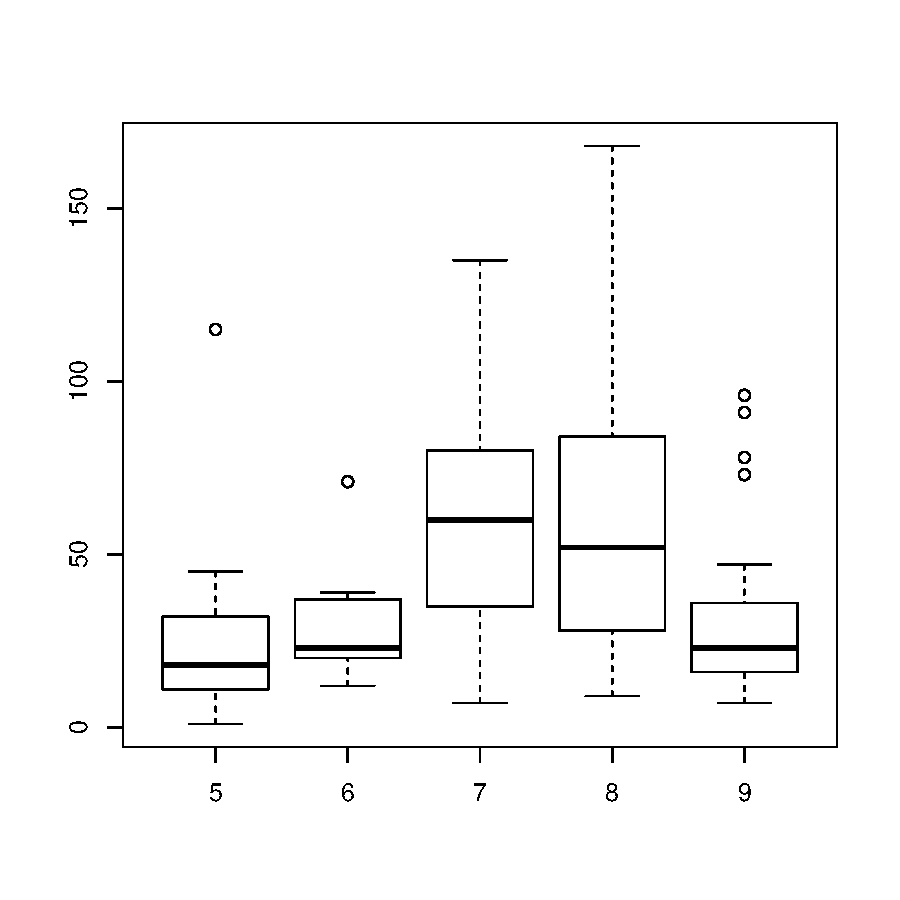
\includegraphics{Assignment_4-004}

heiheiheiiiiiiiiiiiiiiiii
\end{center}


\end{document}
